\section{Surface interactions}
\label{sec:surface_interactions}
We remember from section \ref{sec:slip_length} that the effects of surface interactions become significant as the pore sizes decrease. For very small pores, the number of atoms near the surface is comparable to total number of atoms. In an atomic model that calculates forces, these effects are already taken care of through the atomic forces, but in DSMC, we need a surface interaction model. In this section, we discuss three different models. The main property of these models is to perform a statistically correct transfer of energy and momentum between the surface and the colliding particles. There are two important parameters that incorporate the differences between gases and surfaces of various types; the normal and tangential accommodation coefficients.
\subsection{Accommodation coefficients}
\label{sec:accomodation_coefficients}
When a particle with energy $E_i$ hits a surface, some of the energy might be transferred to the wall resulting in an energy change $\Delta E$. On average, we can define the \textit{normal accommodation coefficient} 
\begin{align}
	\sigma_n = \frac{E_i - E_r}{E_i - E_w},
\end{align}
where $E_i$ is the energy of the incoming particles, $E_r$ is the energy of the outgoing particles and $E_w$ is the energy corresponding to the surface temperature $T_w$. A thermal accommodation coefficient equal to zero would mean that there is no energy exchange, and we will get the specular wall model described below. $\sigma_n=1$ on the other hand means that all the reflected particles have energies corresponding to the surface temperature. This is what we call the thermal wall (or diffuse reflection\cite{karniadakis2005microflows}), and there is no correlation between the incoming and outgoing velocities. More intricate models may use other values of the accomodation coefficients so the particles \textit{remember} their incoming velocities. We can also define the \textit{tangential momentum accommodation coefficient}
\begin{align}
	\sigma_t = {\tau_i - \tau_r\over \tau_i - \tau_w},
\end{align}
where $\tau_i$ and $\tau_r$ are the incoming and outgoing tangential momentum and $\tau_w$ is the momentum of the surface (e.g. a moving surface). 

\subsection{Specular wall}
The specular wall behaves just like how a classical mirror reflects light. The colliding particles are reflected so that the normal component of the velocity is reversed while the tangential components remain unchanged. This leads to the famous saying; \textit{the angle of incidence equals the angle of reflection}. Since the magnitude of all momentum components are unchanged, there is no exchange of energy with the wall. 

\subsection{Thermal wall}
If we instead think of the wall as a reservoir with a given temperature $T_w$, we can imagine that the particles go into the wall, collide with the wall atoms for a while, and at some point, return with no correlation with the incoming velocity. In principle, the outgoing particles doesn't have to be the same as those that go into the wall, but as long as there is no net particle flux we might as well assume this for simplicity. Once a particle has hit the surface, we can choose a new, random velocity vector from a distribution so that the reflected particles have an average velocity according to the wall temperature. Since faster particles collide with the wall more often (this would also be true if we got \textit{new} particles from the reservoir), this distribution has to reflect this fact. A distribution that satisfies this property is the \textit{biased} Maxwell-Boltzmann distribution\cite{alexander1997direct} 
\begin{align}
	P_n(v_n)\dm v_n = {m\over k_BT_w}v_n e^{-\frac{mv_n^2}{2k_BT_w}} \dm v_n,
\end{align}
for the velocity component normal on the surface and
\begin{align}
	P_t(v_t)\dm v_t = \sqrt{m\over 2\pi k_BT_w}e^{-\frac{mv_t^2}{2k_BT_w}} \dm v_t,
\end{align}
for the tangential component. Here $m$ is the mass of the particle and $k_B$ is Boltzmann's constant as usual. However, this distribution does not obey detailed balance since the incoming velocity is completely uncorrelated to the outgoing velocity, but it turns out that it provides great theoretical insight given its simple mathematical form. This, in addition to that it is computationally inexpensive (see section \todo{write it}), it is much used in the literature. 
\subsection{The Cercignani-Lampis model}
A more realistic model is the Cercignani-Lampis model which can be derived requiring detailed balance and wall isotropy (i.e. given incoming velocity $\vec v'$ and outgoing velocity $\vec v$, $P(\vec v' \rightarrow \vec v)$ is unchanged if $\vec v'$ and $\vec v$ are rotated with the same angle about the surface normal vector) \cite{cowling1974cercignani}. The probability of going from an incoming velocity $\vec v'$ to an outgoing velocity $\vec v$ is given as
\begin{align}
	\nonumber
	P(\vec v'\rightarrow \vec v) &= \frac{2\sigma_n\sigma_t(2-\sigma_t)\beta_w^4}{\pi}\\
	\nonumber
	&\times\exp\Big(-\beta_w^2\frac{v_n^2 + (1-\sigma_n)(v_n')^2}{\sigma_n} - \beta_w^2\frac{(v_t - (1 - \sigma_t)v_t')^2}{\sigma_t(2 - \sigma_t)}\Big)\\
	&\times I_0\Big(\beta_w^2\frac{2\sqrt{1 - \sigma_t}v_nv_n'}{\sigma_n}\Big),
\end{align}
where $v_n$ and $v_t$ are the normal and tangential components of the velocities, $I_0$ is the zeroth-order modified Bessel function of the first kind and $\beta_w = (k_BT_w)^{-1}$. $\sigma_n$ and $\sigma_t$ are the accommodation coefficients discussed in subsection \ref{sec:accomodation_coefficients}. We see that the tangential component is a normal distribution with a non-zero mean (the particles remember their incoming velocity), whereas the normal component is more complicated. The normal component distribution is plotted in figure \ref{fig:cercignani_lampis}.
\begin{figure}[h]
\begin{center}
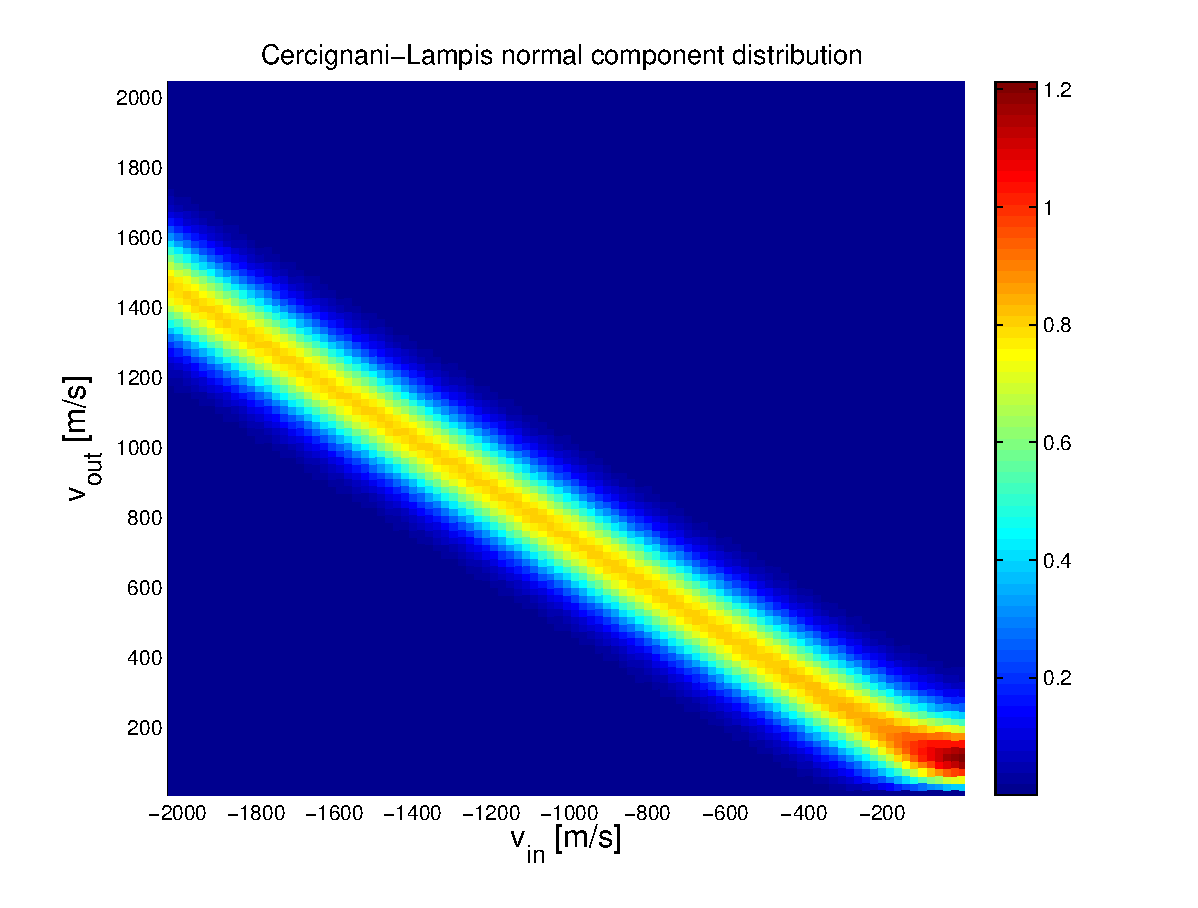
\includegraphics[width=0.85\textwidth, trim=0cm 0cm 0cm 0cm, clip]{DSMC/figures/cercignani-lampis.eps}
\end{center}
\caption{The Cercignani-Lampis normal component distribution for $T_w=\unit{100}{\kelvin}$, $m=\unit{39.948}{\atomicmassunit}$ (argon), $\alpha_n=0.5$. We see that particles with high velocities are on average reflected with a slightly lower velocity, converging towards the velocity corresponding to the wall temperature $T_w$. The mean velocity for this temperature is $\langle v \rangle = $\unit{144}{\meter\per\second}.}
\label{fig:cercignani_lampis}
\end{figure}
\\
To draw random numbers from this distribution is orders of magnitudes slower than that of the thermal wall, since it isn't trivial (if even possible) to invert the cumulative distribution function. Instead we must use the von Neumann algorithm which is a accept-reject Monte Carlo algorithm\cite{allen1989computer}. Our main focus in this thesis is to validate the DSMC model by comparing it to theoretical results of which most have used the thermal wall. The Cercignani-Lampis model is available in the DSMC-code, but due to its computational cost and the low number of comparable theoretical results, we have used the thermal wall in all of our simulations. 